\documentclass[a4paper, 11pt]{scrreprt}
\usepackage[utf8]{inputenc}
\usepackage{graphicx} %% to display pictures by using the \includegraphics command
\usepackage{subfig} %% enable subfigures
\usepackage{float} %% to use the [H] option for graphics
\usepackage[table]{xcolor} %% colors in tables
%\usepackage{xcolor, soul} %% colors and highlighting \hl{} \sl{}

\usepackage{amsmath,amssymb,amsfonts,amstext} %% packages for equations and maths symbols

\usepackage{glossaries} %% make a glossary with abbreviations
\loadglsentries{acronyms} %% load acronyms from acronyms.tex (leave out the filetype)
\makeglossaries %% initialize the glossary

\usepackage{listings}%% package for displaying source code

% define colors for source code list
\definecolor{colKeys}{rgb}{0,0,1}
\definecolor{colIdentifier}{rgb}{0,0,0}
\definecolor{colComments}{rgb}{0,1,0.3}
\definecolor{colString}{rgb}{0,0.5,0}

\definecolor{dkgreen}{rgb}{0,0.6,0}
\definecolor{gray}{rgb}{0.5,0.5,0.5}

%% set options for matlab code
\lstset{			
  language=Matlab,
  keywords={break,case,catch,continue,else,elseif,end,for,function,   global,if,otherwise,persistent,return,switch,try,while,ones,zeros},
   float=hbp,
   basicstyle=\ttfamily\small,
   identifierstyle=\color{colIdentifier},
   keywordstyle=\color{blue},
   commentstyle=\color{green},
   stringstyle=\color{dkgreen},
   columns=flexible,
   tabsize=2,
   %frame=none; %single,
   numbers=left,
   extendedchars=false,
   showspaces=false,
   numberstyle=\ttfamily\small\color{gray},
   stepnumber=1,
   numbersep=10pt,
   showspaces=false,
   showstringspaces=false,
   breakautoindent=true}

\begin{document}
\begin{titlepage} %%creates title page
\centering
	
\includegraphics[width=\textwidth]{graphics/university-logo}\par\vspace{1.5cm}
	\vspace{1.5cm}
	{\scshape\Large Semesterarbeit für das Modul\par
    ModSim2\par
    bei Professorin Dr.\par}
	\vspace{2cm}
	{\huge\bfseries Title\par}
	\vspace{2cm}
	{\Large\itshape Author, MatNr.\par}
	\vfill
	Studiengang:\par
	B.Eng. Maschinenbau\par
    Vertiefungsrichtung Produktentwicklung

	\vfill

	{\large \today\par}
\end{titlepage}
\pagenumbering{Roman} %% capital roman page numbers up to the first chapter

\addcontentsline{toc}{chapter}{Kurzzusammenfassung} %% adds a chapter to the table of content (toc), because the command \chapter* creates a chapter that is not listed in the toc. Thus, it is not numbered to make sure chapter "Introduction" is the first numbered section.
\chapter*{Kurzzusammenfassung}  %Short explanation of project

\newpage
\addcontentsline{toc}{chapter}{Erklärung}
\chapter*{Erklärung}
\vspace{2cm}
Ich versichere hiermit, die von mir vorgelegte Arbeit selbstständig verfasst zu haben. Alle Stellen, die wörtlich oder sinngemäß aus veröffentlichten oder nicht veröffentlichten Arbeiten anderer entnommen sind, habe ich als entnommen kenntlich gemacht. Sämtliche Quellen und Hilfsmittel, die ich für die Arbeit benutzt habe, sind angegeben. \\
Die Arbeit hat mit gleichem Inhalt bzw. in wesentlichen Teilen noch keiner anderen Prüfungsbehörde vorgelegen.\\
\newline
\begin{center}
\vspace{3cm}
\begin{tabular}{ll}
\makebox[6cm]{\hrulefill}\makebox[2cm]{} & \makebox[6cm]{\hrulefill} \\
(Ort, Zeit) & (Unterschrift)
\end{tabular}
\end{center}



%%%%%% Table of Contents %%%%%%  
\newpage
\tableofcontents % make a table of contents
           
\newpage
\addcontentsline{toc}{chapter}{List of Figures}
\listoffigures
      
\newpage        
\addcontentsline{toc}{chapter}{List of Tables}
\listoftables

\newpage
\addcontentsline{toc}{chapter}{List of Acronyms}
\printglossaries %% print the glossary 


\newpage
\pagenumbering{arabic} %% start arabic page numbering
\chapter{Erste Kapitel Ebene}
There is a thing called \gls{cd} and another one called \gls{dvd}.\\
Now only the abbreviations \gls{cd} and \gls{dvd} are displayed.

\section{Zweite Ebene}
lkdcLKDSNvlsknvlkfdnvlyknfdvlkndy

\subsection{Dritte Ebene}
fdsaöljsdlfkmsldfmvlkmfvlkmflkvmslkfm

\section{Zweite Ebene}
adklfjöldsakjfalkdjlaksdjlkajsdlkvcmsdlkm



\newpage
\chapter{Bilder}
How to display pictures:

\begin{figure}[H] %%[H] for "here" so that the picture is not moved to the end of the paragraph
  \centering %% picture is centered
  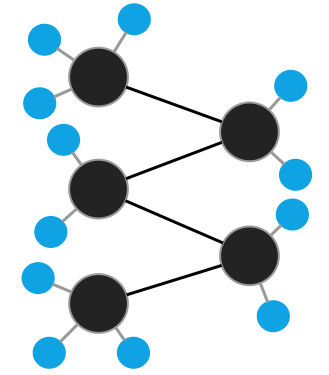
\includegraphics[width=.25\textwidth]{graphics/molecule}
  \caption[Caption for the list of figures]{Caption display below the picture}
  \label{fig:pic1} %% label to reference the picture within the text
\end{figure}
\noindent
Figure \ref{fig:pic1} and \ref{fig:pic2} use the same file. With the command \verb+width=y.x\textwith+ the size can be adjusted.
\begin{figure}[H] %%[H] for "here" so that the picture is not moved to the end of the paragraph
  \centering %% picture is centered
  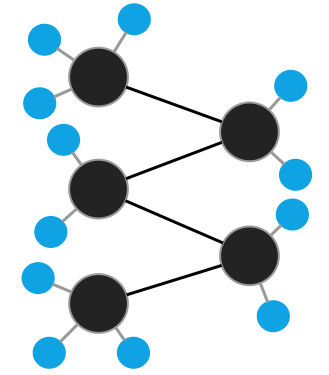
\includegraphics[width=.5\textwidth]{graphics/molecule}
  \caption[Caption for the list of figures]{Caption display below the picture}
  \label{fig:pic2} %% label to reference the picture within the text
\end{figure}
\noindent
\section{Multiple Pictures}
Multiple figures (see Figures \ref{fig:subfig1} and \ref{fig:subfig2} or in general Figure \ref{fig:subfigs}):
\begin{figure}[H]
  \centering
  \subfloat[Subcaption for the first graphic]{
  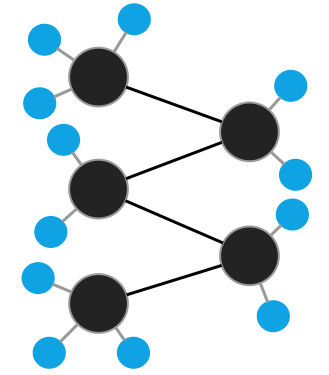
\includegraphics[width=.5\textwidth]{graphics/molecule}
  \label{fig:subfig1}
  }
  \subfloat[Subcaption for the second graphic]{
  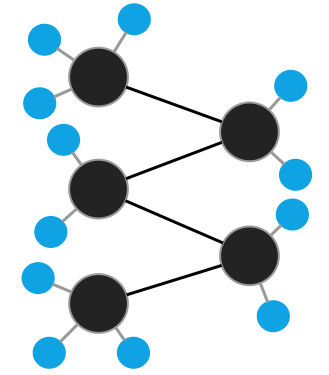
\includegraphics[width=.5\textwidth]{graphics/molecule}
  \label{fig:subfig2}
  }
  \caption[Caption for multiple graphics in the list of figures]{(\ref{fig:subfig1}) Some text for the first graphic. (\ref{fig:subfig2}) Some text for the second graphic.}
  \label{fig:subfigs}
\end{figure}
\noindent
\chapter{Tables}
Super fancy tables.

\begin{center}
\captionof{table}{Combination rules for $\sigma$ and $\varepsilon$ in Gromacs.}\label{table:combination_rules} %% Caption for table and list of tables is the same. The caption needs to be labeled to reference the table.
\begin{tabular}{| c | c | c |}
\textbf{Combination Rule 1} & \textbf{Combination Rule 2} & \textbf{Combination Rule 3} \\
\hline
$W_\mathrm{AA} = 4\varepsilon_\mathrm{A}\sigma^{12}_\mathrm{A}$ & $\varepsilon_\mathrm{A}$ & $\varepsilon_\mathrm{A}$ \\
$V_\mathrm{AA} = 4\varepsilon_\mathrm{A}\sigma^{6}_\mathrm{A}$ & $\sigma_\mathrm{A}$ & $\sigma_\mathrm{A}$ \\
\hline
$W_\mathrm{AB} = \Big( 4\varepsilon_\mathrm{A}\sigma^{12}_\mathrm{A} \cdot 4\varepsilon_\mathrm{B}\sigma^{12}_\mathrm{B} \Big)^{\frac{1}{2}}$ & $\varepsilon_\mathrm{AB} = \sqrt[]{\varepsilon_\mathrm{A}\varepsilon_\mathrm{B}}$ & $W_\mathrm{AB} = \Big( 4\varepsilon_\mathrm{A}\sigma^{12}_\mathrm{A} \cdot 4\varepsilon_\mathrm{B}\sigma^{12}_\mathrm{B} \Big)^{\frac{1}{2}}$ \\
$V_\mathrm{AB} = \Big( 4\varepsilon_\mathrm{A}\sigma^{6}_\mathrm{A} \cdot 4\varepsilon_\mathrm{B}\sigma^{6}_\mathrm{B} \Big)^{\frac{1}{2}}$ & $\sigma_\mathrm{AB} = \frac{1}{2}\big(\sigma_\mathrm{A} + \sigma_\mathrm{B} \big)$ & $V_\mathrm{AB} = \Big( 4\varepsilon_\mathrm{A}\sigma^{6}_\mathrm{A} \cdot 4\varepsilon_\mathrm{B}\sigma^{6}_\mathrm{B} \Big)^{\frac{1}{2}}$ \\
\end{tabular}
\end{center}
\noindent
A simple table showing combination rules for Gromacs (see Table \ref{table:combination_rules}).\\
\verb+\begin{tabular}{| r | l | c |}+ initializes a table with three columns. The entries can be aligned \textbf{r}ight, \textbf{l}eft or \textbf{c}entered. The pipe \verb+|+ creates a vertical line between every cell.\\
\newline

\begin{center}
\captionof{table}{Different row colors}\label{table:diff_row_col}
\rowcolors{2}{green}{pink} %% {starting row}{odd rows}{even rows}
\begin{tabular}{l | c | r}
green & green & green \\
\hline
pink & pink & pink \\
green & green & green \\
pink & pink & pink \\
green & green & green \\
\end{tabular}
\end{center}
\noindent
Use \verb+&+ to separate columns in a row and \verb+\\+ to begin a new row. Table \ref{table:diff_row_col} shows that it is possible to use different colors.

\chapter{Equations}
For equations there are different ways to enter the mathematical environment. Using the command \verb+$ \frac{1}{x} $+ creates $ \frac{1}{x} $ within the text.

\begin{equation}\label{eq:linfnc}
F(x) = m \cdot x + b
\end{equation}

\begin{equation*}
F(x) = ax^{2}+bx+c
\end{equation*}
\noindent
Referencing Equation \ref{eq:linfnc}.\\
\newline
For matrices in brackets use \verb+$\begin{bmatrix} ... \end{bmatrix}$+ :
\begin{center}
$A=\begin{bmatrix}
1	& 0	& \dots	 & 0      \\
0	& 1 	& \dots  & 0 	  \\
\vdots	& 0 	& \ddots & \vdots \\
0 	& \dots & 0	 & 1
\end{bmatrix}$
\end{center}
\noindent
While for matrices in parentheses \verb+$\begin{pmatrix} ... \end{pmatrix}$+ is used :
\begin{center}
$B=\begin{pmatrix}
1	& 0	& \dots	 & 0      \\
0	& 1 	& \dots  & 0 	  \\
\vdots	& 0 	& \ddots & \vdots \\
0 	& \dots & 0	 & 1
\end{pmatrix}$
\end{center}
\noindent 
Using just \verb+$\begin{matrix} ... \end{matrix}$+ yields a matrix without brackets or parentheses:
\begin{center}
$\begin{matrix}
1	& 0	& \dots	 & 0      \\
0	& 1 	& \dots  & 0 	  \\
\vdots	& 0 	& \ddots & \vdots \\
0 	& \dots & 0	 & 1
\end{matrix}$
\end{center}

\chapter{Citations}
To cite something use the command \verb+\cite[page/chapter/..]{label of reference}+\\
For example \cite[Chapter 1]{Cramer2004} or \cite{Dickson2014}.\\
Only references used in the text will be listed in the Reference section. All other information in the bibtex file is left out.

\chapter{Code}
For showing some short code the environment \verb+lstlisting+ can be used.
\begin{lstlisting}[firstnumber=1550]
...
function y = special_function(x, y, options)

  x
  y
  
  y = x+10
  return y
  %adds 10 to x and stores it in y
 ...
\end{lstlisting}
\noindent
This should only be used when important parts of the source code are specifically explained. Complete scripts should be displayed in the \gls{si} (see \ref{SI:matlabsourcecode}).


\newpage
\addcontentsline{toc}{chapter}{References}
\bibliography{mybib.bib} %% file containing the references
\bibliographystyle{unsrt} %% ordered by first appearance 


\newpage
\appendix
\pagenumbering{roman} %% Switch to small roman numbers for the appendix
\chapter{Matlab Source Code}\label{SI:matlabsourcecode}
\lstinputlisting{mfile.m}

\chapter{Source Code Changes}
In the \gls{si} (sub-)sections are possible
\section{Original Source Code}
The original code in mfile.m .
\begin{lstlisting}[firstnumber=100]
...
function y = special_function(x, y, options)

  x
  y
  
  y = x+10
  return y
  %adds 10 to x and stores it in y
  ...
\end{lstlisting}

\section{New Source Code}
Important code changes in mfile.m .
\begin{lstlisting}[firstnumber=100]
...
function y = special_function(x, y, options)

  x
  y
  
  y = x+12
  return y
  %adds 12 to x and stores it in y
  ...
\end{lstlisting}
\end{document}

